\documentclass[b1,portrait]{sciposter}


\usepackage{epsfig}
\usepackage{amsmath}
\usepackage{amssymb}
\usepackage{multicol}
%\usepackage{fancybullets}
\usepackage[brazil]{babel}
\usepackage{ucs}
\usepackage[utf8x]{inputenc}

\newtheorem{Def}{Definition}

%\definecolor{BoxCol}{rgb}{0.9,0.9,0.9}
% uncomment for grey background to \section boxes 
% for use with default option boxedsections

%\definecolor{BoxCol}{rgb}{0.9,0.9,1}
% uncomment for light blue background to \section boxes 
% for use with default option boxedsections

%\definecolor{SectionCol}{rgb}{0,0,0.5}
% uncomment for dark blue \section text 






\title{Boinc + R : Executando rotinas de bioinformática em grades oportunistas}

% Note: only give author names, not institute
\author{Rodrigo L. M. Flores \\ Orientador: Roberto Hirata Jr.}
 
% insert correct institute name
\institute{Instituto de Matemática e Estatística\\
           Universidade de São Paulo\\}

\email{\{flores, hirata\}@ime.usp.br}  % shows author email address below institute

%\date is unused by the current \maketitle


% The following commands can be used to alter the default logo settings
\leftlogo[1.5]{logo_siicusp}  % defines logo to left of title (with scale factor)
\rightlogo{cnpq}  % same but on right

% NOTE: This will require presence of files logoWenI.eps and RuGlogo.eps, 
% or other supported format in the current directory  
%%%%%%%%%%%%%%%%%%%%%%%%%%%%%%%%%%%%%%%%%%%%%%%%%%%%%%%%%%%%%%%%%%%%%%%%%%%%%%%%
%%% Begin of Document

\begin{document}
%define conference poster is presented at (appears as footer)

\conference{{\bf Siicusp 2009}, Siicusp 17 - São Carlos - SP}

%\LEFTSIDEfootlogo  
% Uncomment to put footer logo on left side, and 
% conference name on right side of footer

% Some examples of caption control (remove % to check result)

%\renewcommand{\algorithmname}{Algoritme} % for Dutch

%\renewcommand{\mastercapstartstyle}[1]{\textit{\textbf{#1}}}
%\renewcommand{\algcapstartstyle}[1]{\textsc{\textbf{#1}}}
%\renewcommand{\algcapbodystyle}{\bfseries}
%\renewcommand{\thealgorithm}{\Roman{algorithm}}

\maketitle

\renewcommand{\papertype}{b1}

%%% Begin of Multicols-Enviroment
\begin{multicols}{2}

%%% Abstract
\begin{abstract}
Rotinas de bioinformática são muitas vezes escritas na linguagem \textit{R} que já possui
muitas bibliotecas para análise e desenho de gráficos. Porém, muitas destas rotinas são
combinatórias, o que demanda bastante recurso computacional. O objetivo deste trabalho é,
utilizando uma rede de computadores do IME-USP, criar uma grade computacional para processamento 
destas rotinas, utilizando o renomado middleware \textit{BOINC} como \textit{middleware} para
a distribuição das rotinas.

\end{abstract}

%%% Introduction
\section{Introdução e Objetivos}

\PARstart{A}lgoritmos da área de bioinformática normalmente são combinatórios e bastante custosos computacionalmente
e muitas vezes seu processamento em um único computador pessoal se torna inviável e demorado. A utilização de um 
\textit{supercomputador} pode ser uma boa opção, mas tais tipos de computadores são específicos e caros, o que 
dificulta bastante seu uso. Uma outra opção é utilizar a computação oportuna em grades de computadores de 
uma universidade ou empresa, já que estas normalmente possuem muitos computadores que normalmente ficariam desligados
 em períodos fora do expediente ou sub-utilizados no período de expediente. 

Como já existem muitas bibliotecas para desenvolvimento de aplicações de bioinformática na linguagem \textit{R}, um dos
requisitos do trabalho é fazer com que rotinas nesta linguagem possam ser executadas na grade, evitando assim 
a reimplementação dos algoritmos e programas. 

Para o gerenciamento da grade, utilizamos o já renomado \textit{middleware} \emph{BOINC}, já utilizado em diversos projetos
de computação em grade voluntária (pessoas voluntariamente doando ciclos de CPU para projetos ) e que vem também sendo utilizado
em diversos projetos de computação em grade como o citado em \cite{boinc}.

O objetivo deste trabalho é criar uma grade de computadores na rede CEC do IME-USP utilizando o \textit{BOINC} para distribuir as tarefas
entre os computadores.




\section{Metodologia}

O trabalho consistiu primeiramente no estudo das diversas tecnologias na qual o \textit{R} possui suporte
para processamento em grade. Foi estudado o artigo \cite{Dias}
que havia feito algo parecido utilizando o \textit{middleware} \textit{Alchemi} que funciona na plataforma .NET
da Microsoft. Outro artigo \cite{epub8991}
fazia uma comparação sobre as diversas tecnologias de computação de alta performance no \textit{R}. Por fim, o artigo \cite{boinc}
contava da experiência do uso do \textit{BOINC} em uma universidade da Espanha para processamento em grade. Como
esta última experiência foi bem sucedida, decidimos utilizar o \textit{BOINC} para o gerenciamento de nossa grade.

Como a API do \textit{BOINC} só funciona para C,C++,Java e Python, foi utilizado um \textit{Wrapper} que é um programa distribuído junto com o 
\textit{BOINC} e que executa um arquivo binário, seguindo as instruções fornecidas em um arquivo XML. Para rodar os programas em R,
colocamos como parâmetro um outro programa que apenas chama a função do C system, usando como parâmetro o caminho 
do interpretador junto com o script. 

Escolhido o \textit{middleware}, nos preocupamos em colocar em funcionamento o processamento de rotinas na linguagem R
através do \textit{BOINC}, tanto em ambientes Linux como em ambientes Windows. Para o ambiente Linux o processo foi mais 
simples: havia uma maneira simples de processar trabalhos sem ter que utilizar todo o protocolo de arquivos de entrada e saída
de um \textit{workunit} do \textit{BOINC}. Já para o Windows o processo foi mais trabalhoso: foi descoberto um bug nas configurações 
de compilação do Wrapper e foi necessário uma correção de um desenvolvedor do Boinc. Após isso, foi configurando um servidor
com um projeto do \textit{BOINC} e uma rotina em \textit{R} que faz várias contas para ser testado na grade do CEC. 

\section{Funcionamento do BOINC com a linguagem \textit{R}}

\begin{figure}[!h]
  \centering
  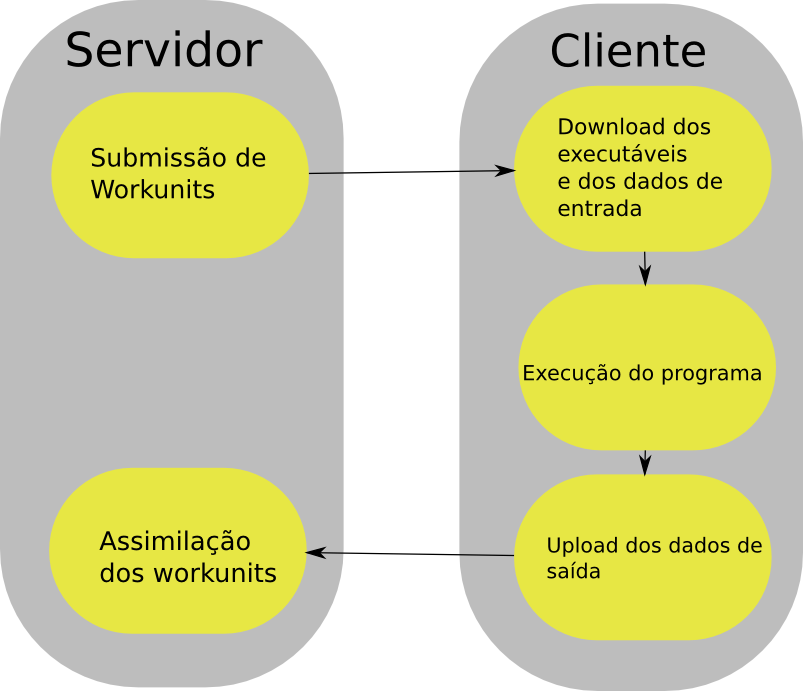
\includegraphics[scale=0.5]{boinc-schema.png}
  \caption{Funcionamento do i\textit{BOINC}}
  \label{boinc_funcionamento}
\end{figure}

O \textit{BOINC} funciona da seguinte maneira: criado um \textit{workunit} que é um conjunto de dados de entrada para uma aplicação, 
o cliente se conecta no servidor, faz o download dos arquivos executáveis da aplicação e dos dados de entrada. Após isso, 
os executáveis são executados com os arquivos de entrada. Quando o processamento acaba, o cliente faz o upload da saída
e o servidor faz a assimilação da saída, colocando as informações em um banco de dados. O funcionamento do Boinc pode ser visto 
na \ref{boinc_funcionamento}.


\begin{figure}[!h]
  \centering
  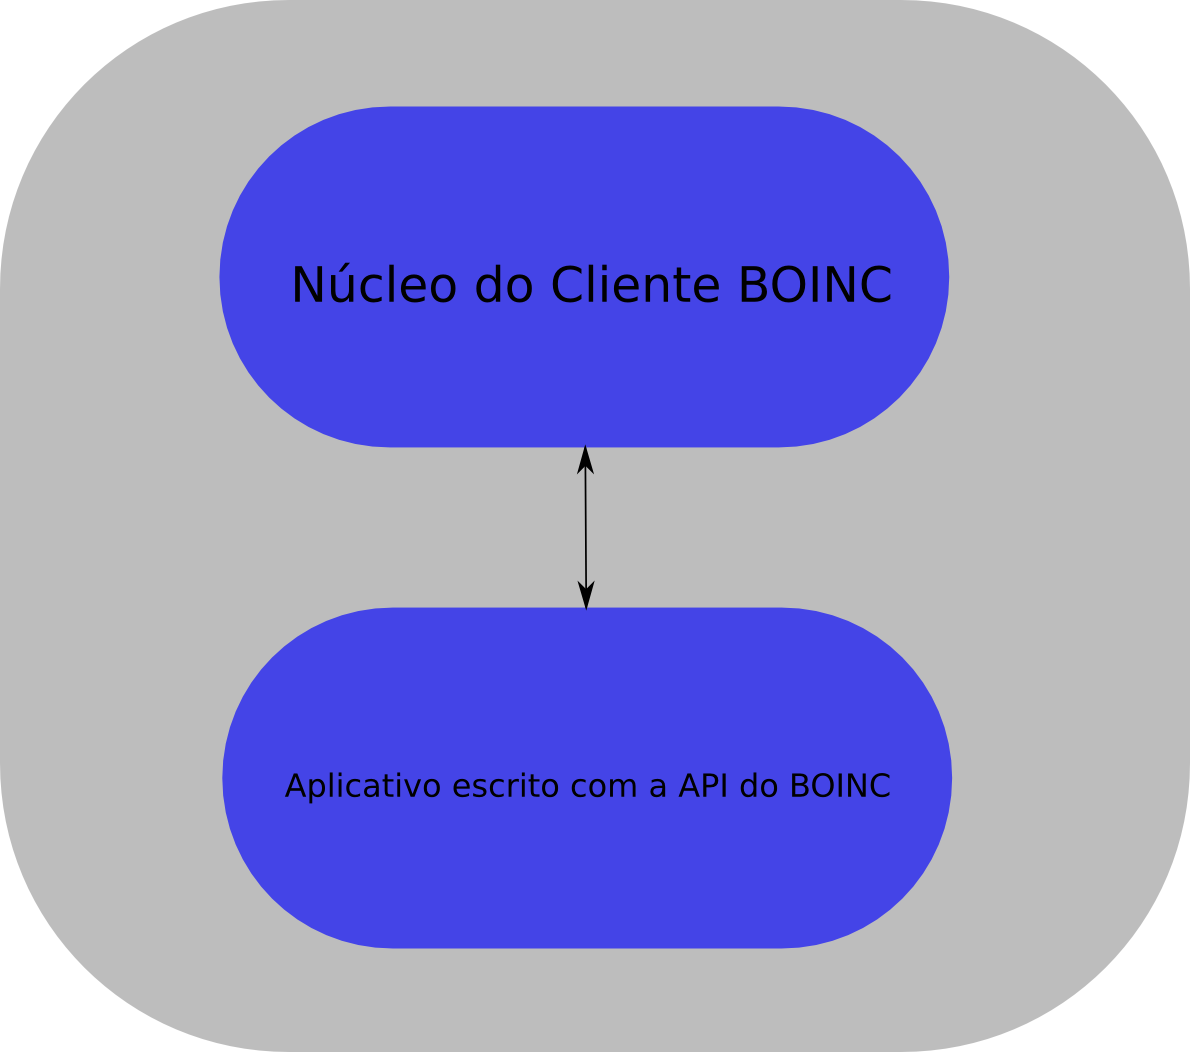
\includegraphics[scale=0.3]{boinc-diagram-normal.png}
  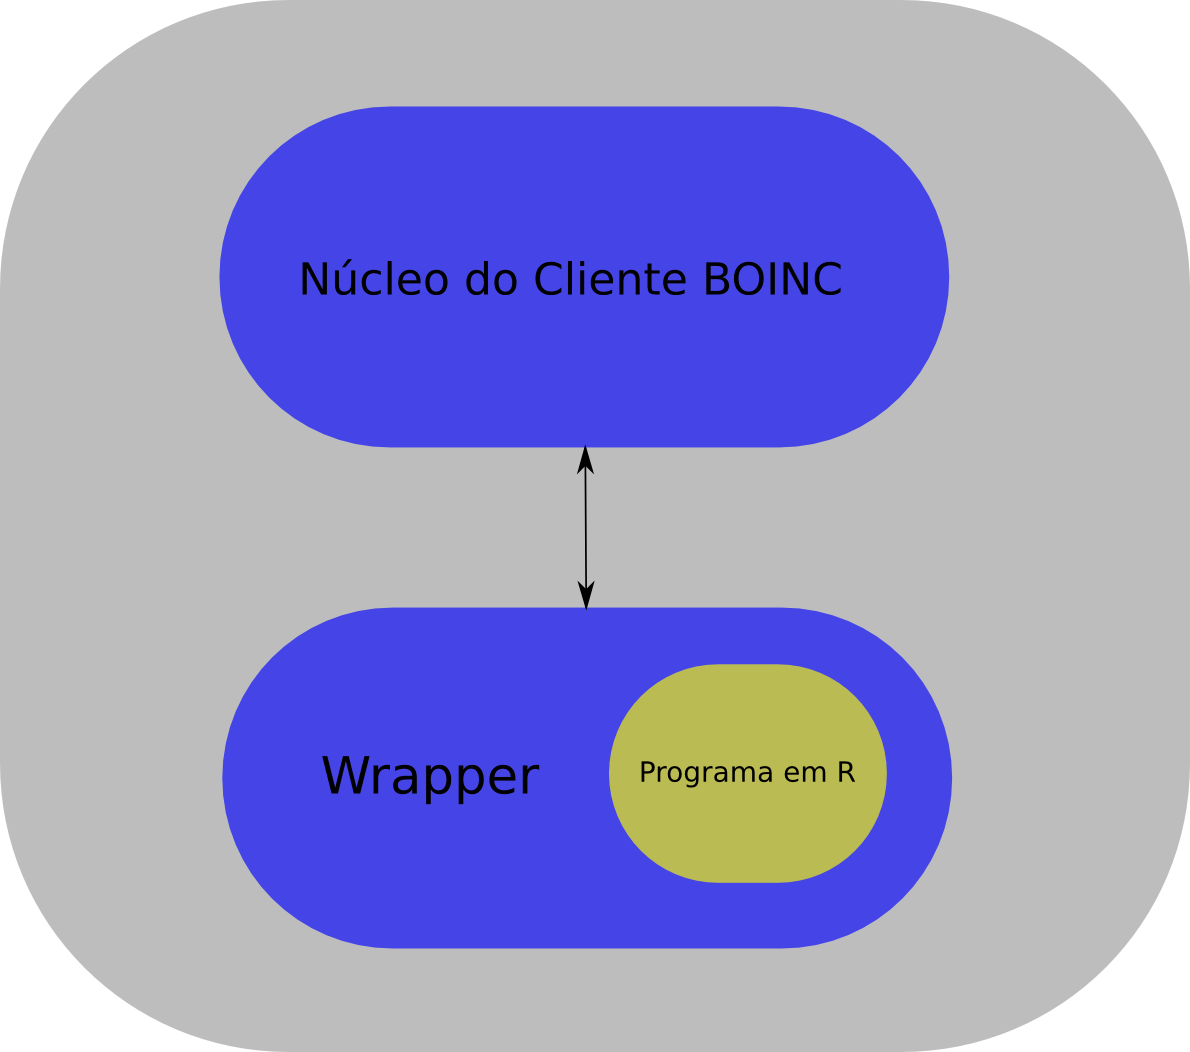
\includegraphics[scale=0.3]{boinc-diagram-wrapper.png}
  \caption{Funcionamento do \textit{BOINC} normal e com o \textit{Wrapper}}
  \label{boinc_funcionamento_nw}
\end{figure}


Aplicações escritas para serem executadas em uma grade gerenciada
pelo \textit{BOINC} são feitas usando a API do  \textit{BOINC}. Porém, como não existe
um \textit{binding} da API do BOINC para a linguagem \textit{R}, 
para a execução de programas nesta linguagem somos obrigados a utilizar
um wrapper. Um wrapper é um programa feito utilizando a API do BOINC
que lê um arquivo XML com as informações de execução de um programa
e o wrapper executa esse programa.  

Utilizando o wrapper, colocamos como parâmetro um programa em C 
que chama o interpretador \textit{R} junto com o programa em \textit{R}
que queremos executar. É necessário que tanto o wrapper
quanto o programa em C sejam compilados para a plataforma na qual será executado. 
Já o interpretador e os arquivos de entrada são os mesmos para ambos os sistemas.

\section{Resultados e discussão}

A parte do servidor já está implementado e em funcionamento. A instalação
dos clientes está em fase de implantação na Rede CEC do IME-USP e em breve 
a grade estará em seu pleno funcionamento.

\section{Conclusão}
 
O objetivo está bem próximo de ser concluído: só é necessário terminar a implantação
na rede e fazer o anúncio pedindo trabalhos para serem executados na grade. Outro ponto
interessante é que é possível ajudar no processamento usando tanto máquinas com sistemas
Linux quanto Windows o que não foi feito nos outros trabalhos semelhantes citados no projeto.  
 
%%% References

%% Note: use of BibTeX als works!!

\bibliographystyle{amsalpha}
\bibliography{bibliografia}


\end{multicols}

\end{document}

